% Section 1. Sources: 607_bounds_paper/paper.tex (history, problem statement), ledger/STATE.md and
% ledger/facts.json (rows mu upper, mu lower), 1201_upper_structures/runs/r9_run2_verify.json (exact R),
% 1251_referee_upper_12297/FINAL.md, 1228_combined_lower/FINAL.md, 1252/1253 FINAL.md.
%%%%%%%%%%%%%%%%%%%%%%%%%%%%%%%%%%%%%%%%%%%%%%%%%%%%%%%%%%%%%%%%%%%%%%%%
\section{Introduction}\label{sec:intro}
%%%%%%%%%%%%%%%%%%%%%%%%%%%%%%%%%%%%%%%%%%%%%%%%%%%%%%%%%%%%%%%%%%%%%%%%

\subsection{The problem}

A meander of order $n$ is a closed road that crosses a straight river $2n$ times and never crosses itself. Two drawings
are the same meander if one can be deformed into the other without changing the order of the crossings. Their number
is $M_n$:
\[ M_1, M_2, \ldots \;=\; 1,\ 2,\ 8,\ 42,\ 262,\ 1828,\ 13820,\ 110954,\ \ldots \]
Figure~\ref{fig:cut} shows one of the $8$ meanders of order $3$; it is the running example of this paper. No formula
for $M_n$ is known. The limit $\mu=\lim M_n^{1/n}$ exists~\cite{AP}, and series analysis of the exact counts gives
$\mu\approx 12.262874$~\cite{JG}. This value is a numerical estimate, not a proved bound. Paper~A of this series~\cite{PaperA} explains why the
problem is hard and what is expected; Paper~C~\cite{PaperC} studies the factor $M_n/\mu^n$ and Paper~D~\cite{PaperD}
a continuum model. This paper proves bounds on $\mu$.

\begin{figure}[htb]
\centering
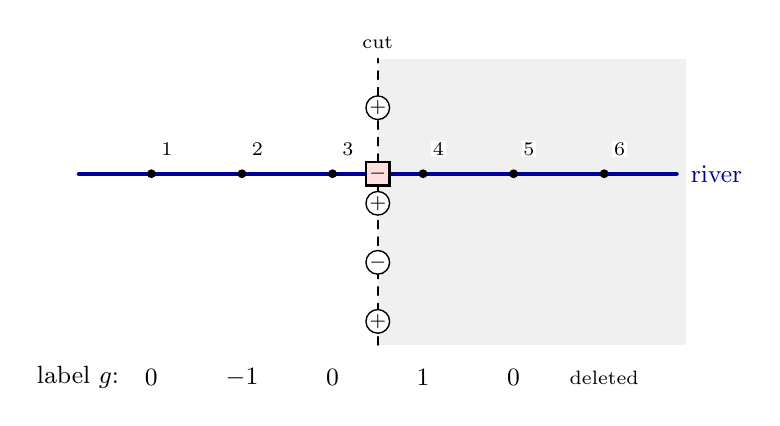
\begin{tikzpicture}[x=1.15cm,y=0.75cm,line cap=round]
  \fill[black!6] (3.5,-2.9) rectangle (6.9,1.95);
  \draw[blue!60!black,line width=1.6pt] (0.2,0)--(6.8,0);
  \node[blue!60!black,anchor=west] at (6.85,0) {\small river};
  \begin{scope}[black!22,line width=0.7pt]\meanderroad\end{scope}
  \begin{scope}\clip (0.2,-2.9) rectangle (3.5,1.95);
    \begin{scope}[line width=1.1pt]\meanderroad\end{scope}\end{scope}
  \draw[dashed,line width=0.6pt] (3.5,-2.9)--(3.5,1.95);
  \node[font=\scriptsize,anchor=south] at (3.5,1.95) {cut};
  \foreach \k in {1,...,6} {\fill (\k,0) circle[radius=1.6pt];
    \node[fill=white,inner sep=0.6pt,font=\scriptsize] at (\k+0.17,0.42) {\k};}
  % signs of the strands met by the cut, bottom to top: + - + [-] +
  \foreach \yy/\s in {-2.5/+,-1.5/-,-0.5/+,1.118/+} {
    \draw[fill=white,line width=0.5pt] (3.5,\yy) circle[radius=0.15cm];
    \node[font=\scriptsize,inner sep=0pt] at (3.5,\yy) {$\s$};}
  \draw[fill=red!13,line width=0.8pt] (3.5,0) ++(-0.15cm,-0.15cm) rectangle ++(0.3cm,0.3cm);
  \node[font=\scriptsize,inner sep=0pt] at (3.5,0) {$-$};
  % labels of the crossings
  \node[anchor=east,font=\small] at (0.75,-3.45) {label $g$:};
  \foreach \k/\g in {1/0,2/-1,3/0,4/1,5/0} {\node[font=\small] at (\k,-3.45) {$\g$};}
  \node[font=\scriptsize] at (6,-3.45) {deleted};
\end{tikzpicture}

\smallskip
{\small tape $+-+[-]+$\qquad stacks $\sigma=(0,-1,0)$, $\tau=(0)$\\
gap numbers from bottom to top $-1,0,-1,0,-1,0$}
\caption{The running example, a meander of order $3$, with the cut after crossing $3$ and the part to the right covered
(gray). The cut meets three unfinished arches below the river, the river, and one unfinished arch above. Reading their
signs from bottom to top gives the tape; the square marks the head on the river. Below the drawing are the labels $g$
of the crossings; crossing $6$ is deleted when labels are assigned. Labels, stacks, gap numbers and tapes are defined
in Section~\ref{sec:tape}.}
\label{fig:cut}
\end{figure}

\subsection{Previous bounds and the main result}

Albert and Paterson proved $11.380\le\mu\le12.901$ in 2005~\cite{AP}. In 2026 Fox released code with certified bounds
$11.6080\le\mu\le12.6319$~\cite{Fox}, and Caroppo, Da~Lozzo, Di~Battista and Vihrovs stated $\mu\le12.806$ in a
preprint~\cite{CDDV}. Earlier in this project a weight method on an encoding of meanders by bracket words gave
$12.0535\le\mu\le12.4147$~\cite{BoundsPaper}. Table~\ref{tab:history} and Figure~\ref{fig:history} collect these
bounds. All bounds in the table are proved; the value $12.2629$ is not.

\begin{theorem}\label{thm:main}
Let $R_+$ be the rational number stored in the upper-bound certificate of Section~\ref{sec:upper}; its numerator and
denominator have $111$ digits, and $R_+=3.50669842637333\ldots<3506698427/10^9$. Then
\[ \frac{6109550428547}{500000000000} \;=\; 12.219100857094 \;\le\; \mu \;\le\; R_+^2 \;=\; 12.29693385352921289818\ldots \]
In particular $12.2191\le\mu\le12.2970$. Moreover $M_n\le R_+^{\,2n-2}$ for every $n\ge1$.
\end{theorem}

The interval has width $0.0778$ and contains the estimate $12.2629$, which lies $0.0438$ above the lower bound and
$0.0341$ below the upper bound.
% Arithmetic: 12.262874-12.219100857 = 0.043773; 12.296933854-12.262874 = 0.034060; width 0.077833 (1228 FINAL: 0.077832997).

\begin{table}[htb]
\centering
\begin{tabular}{llll}
\toprule
lower bound & upper bound & source & method \\
\midrule
$11.380$ & $12.901$ & Albert and Paterson, 2005~\cite{AP} & subclasses; clusters\\
$11.6080$ & $12.6319$ & Fox, 2026~\cite{Fox} & selected states; forgetting\\
 & $12.806$ & Caroppo et al., 2026~\cite{CDDV} & (not examined here)\\
$12.0535$ & $12.4147$ & this project, earlier~\cite{BoundsPaper} & window weights\\
$12.2191$ & $12.2970$ & this paper & tape machine\\
\bottomrule
\end{tabular}
\caption{Bounds on $\mu$. The last column names the method of each source in a few words. The numerical estimate
is $12.2629$.}
\label{tab:history}
\end{table}

\begin{figure}[htb]
\centering
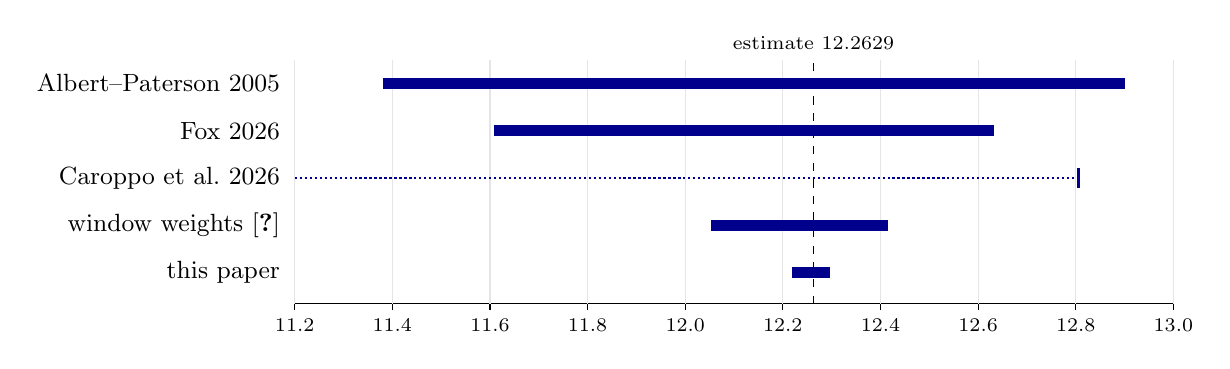
\begin{tikzpicture}[x=6.2cm,y=0.5cm]
  % axis from 11.2 to 13.0
  \draw[line width=0.5pt] (11.2,-5.6)--(13.0,-5.6);
  \foreach \v in {11.2,11.4,11.6,11.8,12.0,12.2,12.4,12.6,12.8,13.0} {
    \draw (\v,-5.6)--(\v,-5.75); \node[font=\scriptsize,anchor=north] at (\v,-5.75) {\v};
    \draw[black!10] (\v,-5.6)--(\v,0.6);
  }
  \draw[dashed,line width=0.6pt] (12.2629,-5.6)--(12.2629,0.6);
  \node[font=\scriptsize,anchor=south] at (12.2629,0.6) {estimate $12.2629$};
  % rows
  \foreach \lo/\hi/\y/\name in {11.380/12.901/0/{Albert--Paterson 2005},11.6080/12.6319/-1.2/{Fox 2026},12.0535/12.4147/-3.6/{window weights~\cite{BoundsPaper}},12.2191/12.2970/-4.8/{this paper}} {
    \draw[line width=4pt,blue!55!black] (\lo,\y)--(\hi,\y);
    \node[font=\small,anchor=east] at (11.19,\y) {\name};
  }
  \draw[densely dotted,line width=0.8pt,blue!55!black] (11.2,-2.4)--(12.806,-2.4);
  \draw[line width=1.2pt,blue!55!black] (12.806,-2.65)--(12.806,-2.15);
  \node[font=\small,anchor=east] at (11.19,-2.4) {Caroppo et al.\ 2026};
\end{tikzpicture}
\caption{The bounds of Table~\ref{tab:history} as intervals. The third row has an upper bound only. The dashed line is the
numerical estimate, which is not a bound.}
\label{fig:history}
\end{figure}

\subsection{The methods in outline}

\emph{The tape machine} (Section~\ref{sec:tape}). Cover a meander with a sheet of paper and slide the sheet to the
right, uncovering the crossings one at a time from the left. Where the sheet stops, its edge meets unfinished pieces of
road below the river, the river, and unfinished pieces above. Each of them gets a sign, $+$ or $-$, by a rule
explained in Section~\ref{sec:tape}. Read from bottom to top, the signs form a word, the \emph{tape}, and the letter
of the river is marked as the \emph{head}. Uncovering one more crossing is a \emph{move}: it changes the tape only at
the head and its two neighbors. Meanders of order $n$ correspond exactly to the sequences of $2n-2$ moves that start
and end at the tape $+[-]+$ (the \emph{closed walks}). Tapes can be arbitrarily long, but every move is local, and both
methods use this.

\emph{The upper bound} (Sections~\ref{sec:weights} and~\ref{sec:upper}). If every tape has a positive weight and the
tapes one move later (its \emph{successors}) weigh at most $R$ times as much in total, then there are at most $R^t$
closed walks of $t$ moves. Since a meander of order $n$ takes $2n-2$ moves, this gives $\mu\le R^2$. We use a sharper
form of this test: each tape has a forward and a backward weight, and each move carries a factor whose reciprocal is
carried by the reverse move. The weights are built so that the ratios entering the test depend only on the letters
near the head, so a finite list of cases covers all tapes. The finite data together with the exact check of these cases is the
\emph{certificate}; here and below, a \emph{certified} bound is one proved by such a check.

\emph{The lower bound} (Sections~\ref{sec:flows} and~\ref{sec:lower}). Consider a random rule for the next move that
is stationary, so that the tape seen from the head looks statistically the same at all times, and that on average
neither lengthens the tape nor moves the head toward one end. Such a rule produces about $e^{ht}$ different sequences
of $t$ moves, where $h$ is its entropy per move, and each of them can be completed to a closed walk with few extra
moves. This gives $\mu\ge e^{2h}$. The certificate is such a rule, written as an exact solution of a finite system of
linear equations.

\subsection{Status of the results}

The tape machine (Theorem~\ref{thm:tape}) and both certificates are new in this project. The bijection was proved in
the project, checked in a separate independent reading, and confirmed by counting closed walks up to order $15$. The
upper certificate was checked in exact rational arithmetic by its own checker and by a second checker written
independently from a separate statement of the theorem; that independent reading also re-proved each step from the
certificate to the bound. The lower certificate rests on a theorem about stationary random rules (Theorem~F in
Section~\ref{sec:flows}) and on four constructions that keep the rule exactly stationary; each of these arguments was
re-derived in a separate independent reading, and the computation was reproduced and recomputed with independently
written code. One part of the lower check is a sample, not a complete replay: the linear equations that express
stationarity for the two largest windows hold by construction and were confirmed only on samples
(Section~\ref{sec:checks}). Nothing has been reviewed outside the project, and no proof assistant was used. Programs,
proofs and certificates are in the project repository~\cite{Repo}; Appendix~\ref{app:where} lists where each proof is.

We have not found the tape machine in the literature. Our search was limited, and the general idea of reading a
meander from left to right while keeping the unfinished arches in two stacks is classical; see~\cite{Jensen} for a transfer matrix method of this
kind.
